\section*{Introduction}

\subsection*{Intended Audience}

This document is intended for undergraduates interested in learning more about the Discrete Fourier Transform 
and digital signal processing.  The goal is to present the DFT, a difficult and complicated topic, in an 
intuitive format that shows its use for audio applications.  Where possible I will try and eschew 
cumbersome math.  However, an understanding of math is essential for even a basic understanding of
the Discrete Fourier Transform.  What
math is required?   Readers should have an understanding of trigonometry
and trigonometric identities as well as summation notation, but topics like calculus are unnecessary.  I suspect that
many reading this document already have an understanding of core audio principles like sampling, sampling
rate, aliasing, etc.  Many of these topics can be found in an introductory course on digital audio so I will assume
the reader has familiarity with those topics as well.

\subsection*{Why do we need the Discrete Fourier Transform?}

Before we start examining the Discrete Fourier Transform (abbreviated DFT for the remainder
of this document), we must first motivate why we even need it in the first place.  Sound can be expressed
in two domains: the time domain and the frequency domain.  The former is the more natural way to think 
about sound.  We perceive sound as an evolution over time.  Songs have verses and choruses and those
formal parts happen at specific moments in time.  We simply cannot absorb the entirety of a song in one
instant as we could with a painting.  The time domain representation of sound mimics the way we 
perceive it.  It expresses sound as a fluctuation of amplitude over time where amplitude represents
the change in pressure that are detected by our ears.  In the digital world, the amplitude is represented 
as a sequence of samples.  Each sample contains a measurement of the sound's amplitude, a value 
typically between -1 and 1.

The frequency domain is perhaps a more surprising way to think about sound, though equally valid.  The
frequency domain expresses sound as a set of frequencies where each frequency is modeled as a sinusoid.  
A sinusoid is simply any wave of the form $ A\sin(2\pi f t + \phi)$ where $A$ is the amplitude, $f$ is the 
frequency, and $\phi$ is the phase.\footnote{Note that a 
	cosine wave is also a 
	sinusoid as it is equivalent to a sine wave with a phase shift.
}  It turns out that \textbf{any sound} can be 
decomposed into a sum of sinusoids having fixed amplitude, frequency and phase.  Mathematically then, an
arbitrary sound can be expressed as a sum of the following form:

$$A_1\sin(2\pi f_1 t + \phi_1) + A_2\sin(2 \pi f_2 t + \phi_2) + A_3\sin(2 \pi f_3 t + \phi_3) + ...$$

\noindent Furthermore, if the sound is periodic\footnote{
	Only periodic signals that satisfy the Dirichlet conditions can be decomposed as a sum of harmonics.  
	But for all pratical purposes, any real audio signal will satisfy the Dirichlet conditions.
}  (i.e., that it repeats exactly over the same successive time interval), then 
the sound can be decomposed into a sum of \textbf{harmonic} sinusoids with fundamental frequency $f$:

$$A_1\sin(2\pi f t + \phi_1) + A_2\sin(2 \pi (2)f t + \phi_2) + A_3\sin(2 \pi (3)f t + \phi_3) + ...$$

\noindent  The above conclusion about periodic signals is sometimes referred to as the Fourier Series.

The notion that any sound or signal could be decomposed into a set of frequencies was an amazing 
discovery in the mid-nineteenth century and is attributed to Joseph Fourier after whom the
Discrete Fourier Transform and Fourier Series is named.  What this discovery implies is that you can recreate 
any sound (i.e., a song, 
field recording, speech) by simply summing together a series of sinusoids, assuming the sinusoids have the correct 
amplitudes, frequencies, and phases.  Wild!  The frequency domain, then, is the collection of frequencies, including
their respective amplitudes and phase,
that constitute a sound.   I sincerely hope that you are questioning how it is possible that \textit{any} sound can be
constructed from a set of sine waves.  It is by no means obvious.  Sadly, we will not prove this truth.  
The math is beyond the scope of this document.  We will simply have to take it as gospel and use it to our 
advantage as we progress through our understanding of the DFT.

To show that sound can be decomposed into sine waves, let us take a look at a classic example: the square wave.
The square wave is periodic.  Therefore, it can be decomposed into a sum of harmonic sinusoids with some 
fundamental frequency $f$.  This should feel wrong on some intuitive level.  The
square wave has discontinuities and lines of zero slope.  It would seem impossible that we could take a series of
sinusoids -- let alone sinusoids from a harmonic series -- and sum them to create a square wave.  Yet it is 
true, though it will not be a perfect representation due to the discontinuities.\footnote{This is called the Gibbs
	Phenomenon.} A square
wave can be created by summing the odd harmonics where each harmonic's amplitude is one over 
the harmonic number.

Figure \ref{fig:square} shows an iterative process where each successive plot depicts the next harmonic 
added.  As more and more harmonics get added, the graph begins to move closer to the shape of a square wave.  
This example though illustrates a key point of signal processing, namely that any
periodic waveform can be represented as a sum of harmonic sinusoids.  

\begin{figure}[h]
	\caption{Successive addition of harmonics to approximate a square wave}
	\label{fig:square}
	\begin{center}
		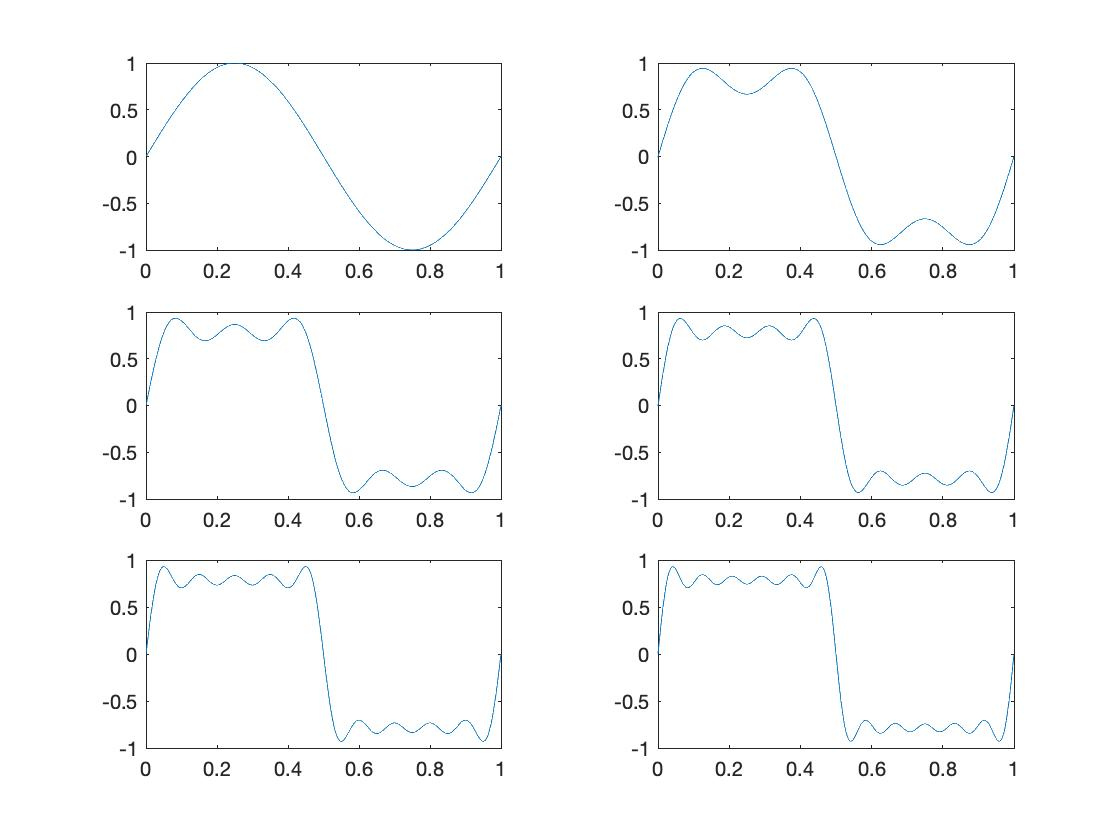
\includegraphics[scale = 0.3]{square.jpg}
	\end{center}
\end{figure}

	We now have two  equally valid ways to think about sound.  One is to consider sound
as a change in amplitude over time.  The other is to consider the various frequencies that make up that sound.  It
may be surpising at first to recognize that the frequency domain makes no consideration of time.  It
feels strange that a series of unchanging sine waves added together can really express the evolution of
sound over time that we experience when we listen to music, but it is indeed true.
	
	But how do we actually figure out the sinusoids that make up a given sound?  The answer: the Discrete Fourier
Transform!  The DFT is a tool to convert a sound from the time domain signal to the frequency domain..  
Once in the frequency domain we can do various spectral manipulations
to change the sinusoidal components of the original sound and convert it back to the time domain using the
Inverse Discrete Fourier Transform (abbreviated as IDFT).  Together the DFT and the IDFT are the two
tools we need to convert between the time domain and frequency domain of any sound.

\subsection*{Getting Our Terminology Right}

You may have heard of several different ``flavors" of tools with the name Fourier in them: Fourier Transform,
Fourier Series, Discrete Fourier Transform, Discrete-Time Fourier Transform, Short-Time Fourier Transform, ... etc.
It is difficult to keep all of these different concepts straight.  Each one though is a tool to convert a time domain
signal to its frequency domain.  The differences lie in whether time is continuous or discrete, whether the
transformation produces a continuous or discrete frequency domain, and whether the time domain signal is 
periodic or aperiodic. 

We perceive sound as a continuous stream over some duration.  It is continuous because at any given instant
we could measure the air pressure processed by our ears.  Recall that we represent air pressure using
amplitude.  Therefore, we can say every instant in time of some sound is associated with a particular 
amplitude.  This is what
is meant by continuous time.  So exactly how many instants of time are there in a given piece of music?
The answer: infinite!  Unfortunately, it is impossible for
digital systems and computers to record the amplitude for every instant in time.  We would need an infinite 
number of amplitudes for our infinite moments in
time to represent every recorded sound properly.  Computers and digital systems can only store a finite amount of data.  Sampling is a compromise for
this limitation.   We can get the overall picture of a sound by 
measuring the amplitude at a small enough period that the original sound can be rendered 
almost exactly the same as the original.  For example, we might sample 30 seconds of a song by taking
a million samples.  Even though a million numbers is quite large, our modern machines can comfortably
store that amount of data.  Sampling generates a finite amount of data, and any finite set of data can be
stored on a computer as long as its not too large.

Similarly, a sound in the frequency domain can be made of an infinite number of sinusoids.  If
we want to store the frequency domain of a sound in a computer, we will only be able to store a subset of those
sinusoids.  It is simply the limitations of the technology we have available to us.  Akin to sampling amplitude,
we want to sample the sinusoids from the frequency domain at a high enough resolution that we can get
an overall sense of its frequency domain.

So why do we care about the Discrete Fourier Transform in particular?  Because it converts a finite discrete
signal (i.e., a finite number of samples) into a finite discrete frequency domain (i.e., a finite number of sinusoids 
with particular phases and amplitudes).  Some of these other tools like the Fourier Transform, for example, take a 
signal of continuous time and convert it to a continuous and infinite frequency spectrum.  Others like the
Discrete-Time Fourier Transform work with infinitely sampled signals and convert them to a continuous frequency
spectrum.  The Discrete Fourier Transform is the practical option for us as musicians because we can process a finite
number of samples from a song say and get an approximate rendering of its sinusoidal components using
a computer.  Courses in
digital signal processing will spend much more time dealing with these other transforms.

One final point.  If you spend enough time studying electronic music or audio technology, you will invariably come
across the Fast Fourier Transform.  The Fast Fourier Transform (abbreviated as FFT) is identical to the Discrete Fourier Transform except
that it is... faster!   The FFT is a way to calculate the computations needed for
the DFT more quickly.  It was one of the most important discoveries in technology in the twentieth century and revolutionized
our ability to process signals in a timely fashion.  Most software and audio programming languages reference
the FFT.  Just know that there is no difference between the FFT and the DFT other than computational speed.
